%%%%%%%%%%%%%%%%%%%%%%%%%%%%%%%%%%%%%%%%%%%%%%%%%%%%%%%%%%%%%%%%%%%%%%%%%%%%%%%%
%% O&P                                                                        %%
%%%%%%%%%%%%%%%%%%%%%%%%%%%%%%%%%%%%%%%%%%%%%%%%%%%%%%%%%%%%%%%%%%%%%%%%%%%%%%%%
\section{O\&P}

% O&P - references
This section introduces the O\&P\footnote{The metamodel was not given a name by its authors; we will, for the purposes of this thesis, call it ``O\&P''.} metamodel described in \cite{Odell01}, \cite{Parunak02}, \cite{Odell03b}, \cite{Odell04b} and \cite{Odell05}.
The overview presented here is due to \cite{Odell05} in particular.

% O%P - authors
O\&P has been put forward in 2001 by James J. Odell, H. van Dyke Parunak and their colleagues.

%% Summary %%%%%%%%%%%%%%%%%%%%%%%%%%%%%%%%%%%%%%%%%%%%%%%%%%%%%%%%%%%%%%%%%%%%%

- PIM

%%%%%%%%%%%%%%%%%%%%%%%%%%%%%%%%%%%%%%%%%%%%%%%%%%%%%%%%%%%%%%%%%%%%%%%%%%%%%%%%
\subsection{Integrated Model}

% Integrated model - about
Figure~\ref{figure:onp-metamodel} shows the integrated model proposed in \cite{Odell05}.
The following subsections will focus on parts of the integrated model that can be studied in isolation.
We present the full model before discussing its parts (ALT: portions, sections) so that the reader can follow the discussion with assumption about where the part fits.

% Figure: O&P metmodel
\begin{figure}[ht]
	\centering
	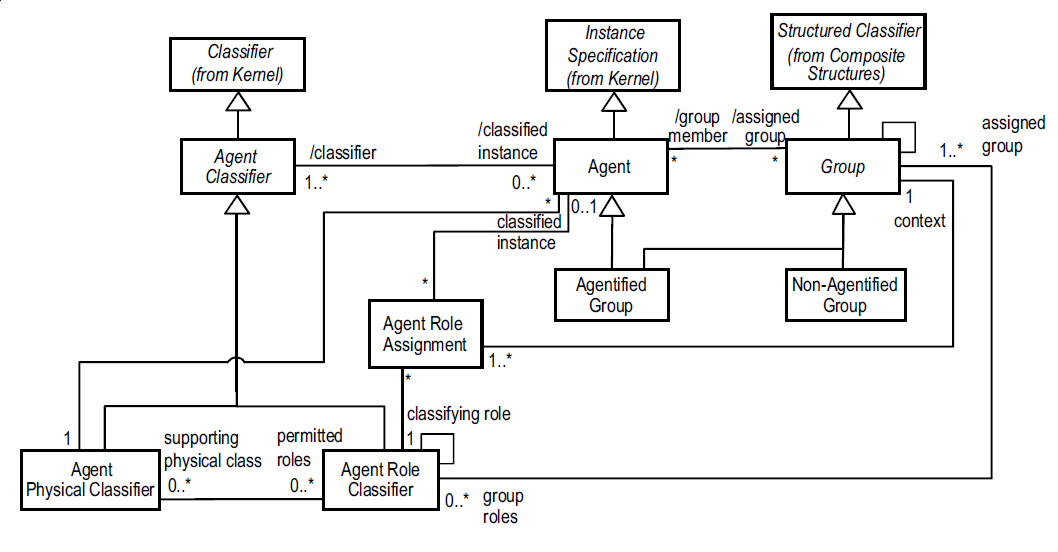
\includegraphics[width=0.75\textwidth]{images/onp/onp-metamodel.png}
	\caption{The O\&P metamodel}
	\label{figure:onp-metamodel}
\end{figure}

% UML Classifier vs. UML Class
To understand the integrated model, it is essential to differentiate between the \textit{Classifier} and the \textit{Class} UML classes.
In short, Classifier does not have features that are associated with a OOP class (e.g. attributes, inheritance or interfaces).
On the other hand, the Class has these features.
Class is in fact a specialization of Classifier.
It is important to make this distinction, because the agent classification is based on an extension of Classifier, not Class.
The reason for this is that the authors did not want to impose object-orientation upon their metamodel.
After all, it is not at all expected of an agent to exhibit behaviour intrinsic to an object (e.g. polymorphism). 

%%%%%%%%%%%%%%%%%%%%%%%%%%%%%%%%%%%%%%%%%%%%%%%%%%%%%%%%%%%%%%%%%%%%%%%%%%%%%%%%
\subsection{Agent Classifiers and Agent}

\textit{Agent Classifier} is a UML Classifier that specifically provides a way to classify Agent instances by a set of features that they have in common \cite{Odell05}.
Classification is important because it enables a common definition of a set of entities that are in some sense similar, i.e. share some features and/or capabilities.

Figure~\ref{figure:onp-agent-classifiers} shows \textsc{Agent Classifier} and its two specializations: \textsc{Agent Physical Specifier} (alias \textsc{Physical Classifier}) and \textsc{Agent Role Specifier} (alias \textsc{Role Classifier}).

\begin{figure}[ht]
	\centering
	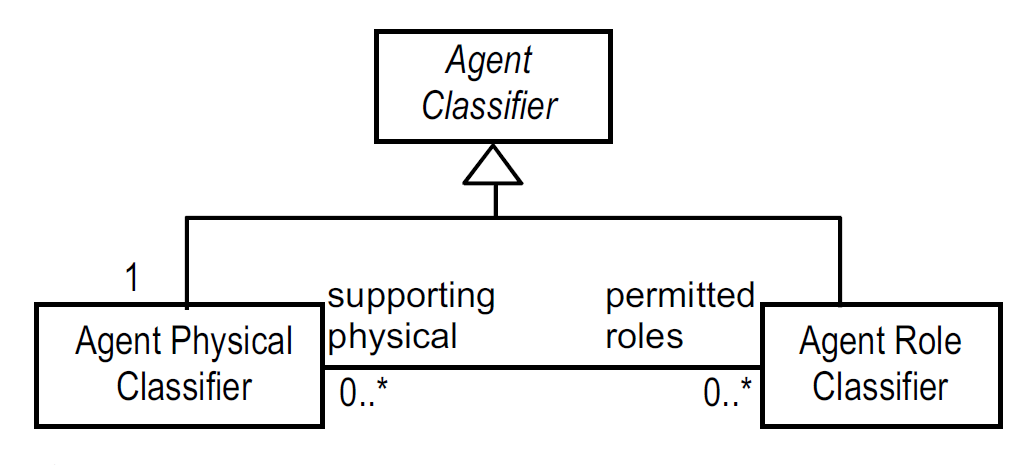
\includegraphics[width=0.5\textwidth]{images/onp/agent-classifiers.png}
	\caption{\textsc{Agent Classifier} and its two specializations: \textsc{Agent Physical Classifier} and \textsc{Agent Role Classifier}}
	\label{figure:onp-agent-classifiers}
\end{figure}

\subsubsection*{Agent Physical Classifier}

% Physical classifier - definition
The purpose of \textsc{Agent Physical Classifier} is to define a set of core features that an agent classified with it has independent of roles it plays \cite{Odell05}.
Every agent must be classified with exactly one physical classifier \footnote{Compare this with OOP, where an object must be an instance of exactly one class.} and is almost never reclassified during its lifetime.

% Physical classifiers vs. role classifiers
Figure~\ref{figure:onp-physical-classifier-examples} illustrates some examples of physical classifiers forming a (class?) hierarchy.
In comparison to role classifiers, physical classifiers attribute primary and permanent features to agents.
An example of a physical classifier from the real world would be `Human' agent.

% Figure: Physical classifer examples
\begin{figure}[ht]
	\centering
	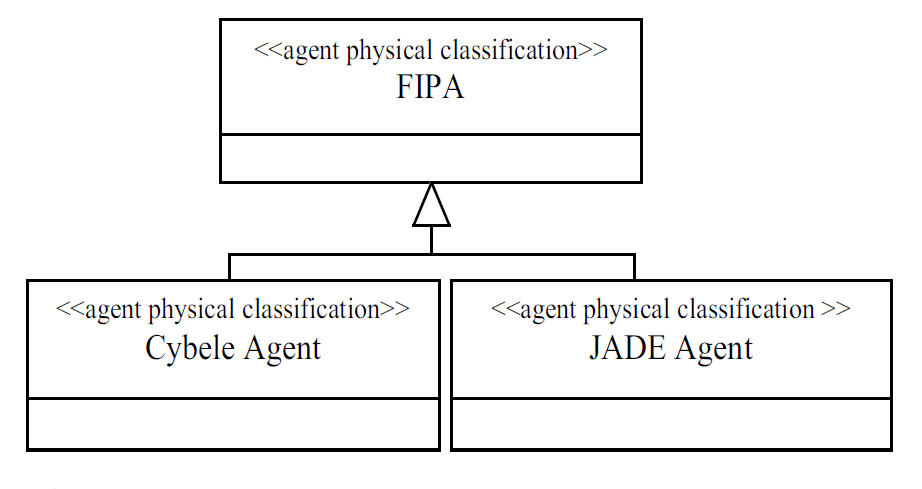
\includegraphics[width=0.5\textwidth]{images/onp/physical-classifier-examples.png}
	\caption{Examples of physical classifiers forming a (class?) hierarchy}
	\label{figure:onp-physical-classifier-examples}
\end{figure}

\subsubsection*{Agent Role Classifier}

% Role classifier - definition
The \textsc{Agent Role Classifier} is a classifier that defines a set of peripheral (as opposed to core) features that an agent classified with it has.
An agent can be classified with more than one role classifier at once (\textit{multiple classification}) and can be reclassified over time (\textit{dynamic classification}).

% Role hierarchy vs. class hierarchy
Figure~\ref{figure:onp-role-classifier-examples} depicts a small (class?) hierarchy of role classifiers.
In AUML, they are marked with the <<agent role>> stereotype.
In comparison to physical classifiers, role classifiers ascribe secondary and transient features to agents.
An example of a role classifier from the real world would be `Chess player' agent.

% Figure: Role classifer examples
\begin{figure}[ht]
	\centering
	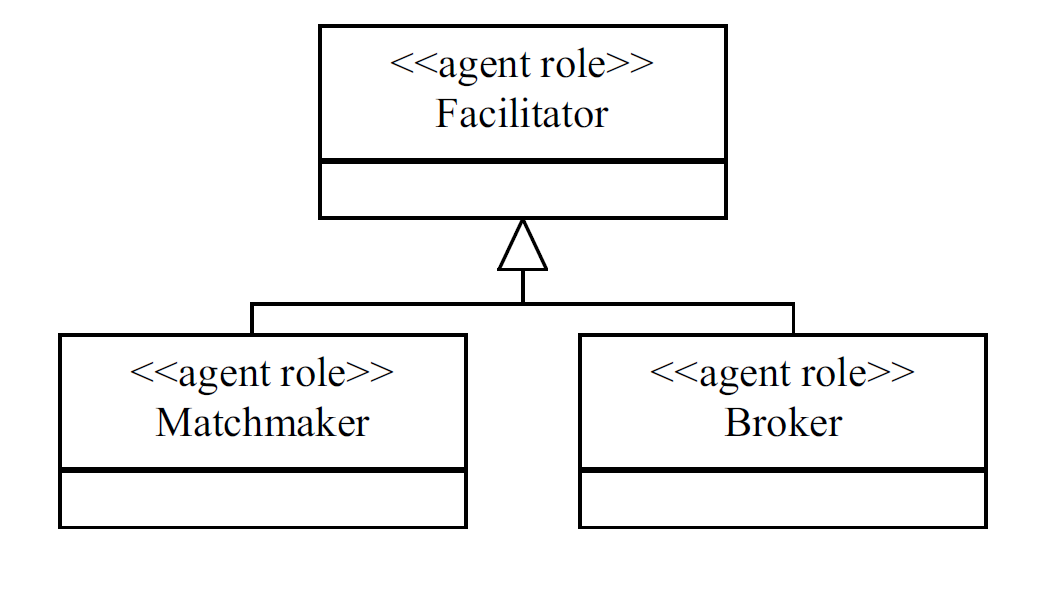
\includegraphics[width=0.5\textwidth]{images/onp/role-classifier-examples.png}
	\caption{Examples of role classifiers forming a (class?) hierarchy}
	\label{figure:onp-role-classifier-examples}
\end{figure}

\subsubsection*{Agent}

In O\&P, the basic concepts are \textsc{Agent Classifier} and \textsc{Agent}.
These modelling constructs are considered fundamental, because they enable a MAS designer to model \textit{agents classes} and \textit{agent instances} respectively.
Agent classes are the design-time (ALT: compile-time?) constructs providing the classification (features) of the actual run-time constructs - agent instances.
Said differently, an agent classifier defines features (state and behaviour) the the associated agents have. 

% TODO: Consider deleting this paragraph.
An \textsc{Agent} instance describes an agent.
This description can be incomplete; the purpose of an \textsc{Agent} instance is to only show what is of interest about an agent in the modelled MAS \cite{Odell05}.

% Figure - about
Figure~\ref{figure:onp-agent-examples} shows two \textsc{Agent} instances: \texttt{Agent4} and \texttt{Agent2}.
Agents may be linked via the roles they play.
In this scenario, \texttt{Agent4} is a broker and brokers something for \texttt{Agent2} who is a seller.

% Figure: Agent examples
\begin{figure}[ht]
	\centering
	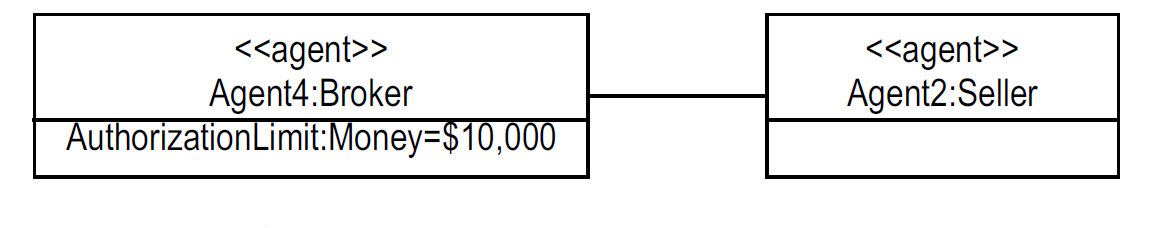
\includegraphics[width=0.5\textwidth]{images/onp/agent-examples.png}
	\caption{Examples of (linked) agents}
	\label{figure:onp-agent-examples}
\end{figure}

\subsubsection*{Association between Agent Physical Classifier and Agent Role Classifier}

The association between \textsc{Agent Physical Classifier} and \textsc{Agent Role Classifier} specifies which role classifiers are permitted for each physical classifier, independent of the capabilities of the individual agents classified with that that particular physical classifier \cite{Odell05}.

Figure~\ref{figure:onp-physical-classifier-role-classifier-association} illustrates the association between \textsc{Agent Physical Classifier} and \textsc{Agent Role Classifier}. It shows instances of \textsc{Agent Physical Classifier}: \texttt{JADE Agent Classifier} and \texttt{Cybele Agent Classifier}; and instances of \textsc{Agent Role Classifier}: \texttt{Manager}, \texttt{Broker}, \texttt{Trust Manager} and \texttt{Buyer}.
The \texttt{JADE Agent Classifier} physical classifier allows the \texttt{Manager} and \texttt{Broker} role classifiers to be played by JADE agents.
Similarly, the \texttt{Cybele Agent Classifier} physical classifier allows the \texttt{Broker}, \texttt{Trust Manager} and \texttt{Buyer} role classifiers to be taken on by Cybele agents.

% Figure: Agent physical classifier to Agent role classifier association
\begin{figure}[ht]
	\centering
	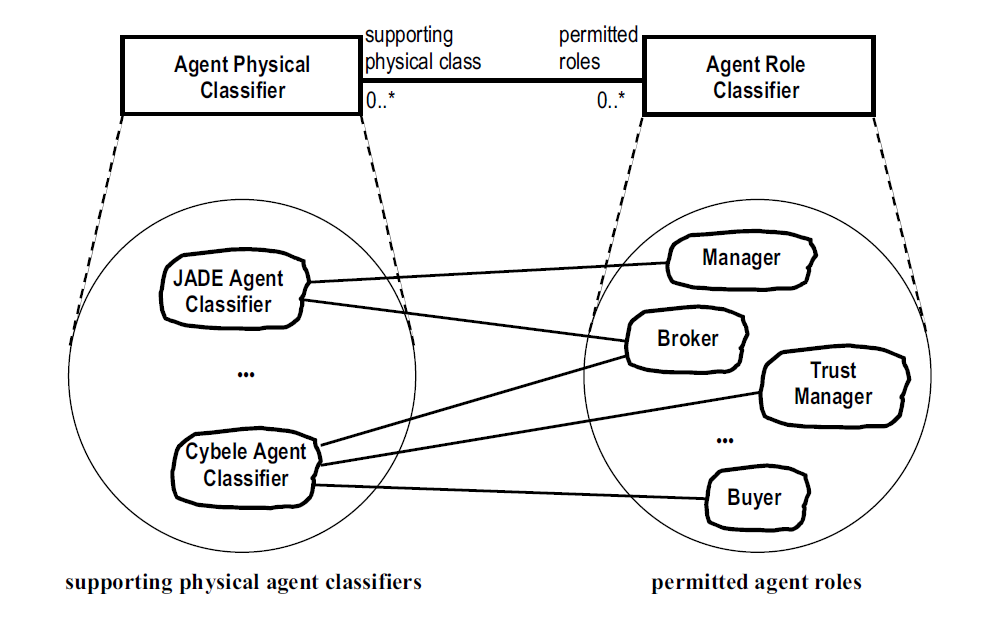
\includegraphics[width=0.75\textwidth]{images/onp/physical-classifier-role-classifier-association.png}
	\caption{The association between \textsc{Agent Physical Classifier} and \textsc{Agent Role Classifie}}
	\label{figure:onp-physical-classifier-role-classifier-association}
\end{figure}

\subsubsection*{Association between Agent and Agent Classifier}

The links of an agent with its agent classifiers (physical and role) determine its features.
Each agent classifier classifies an agent as a member of a set of agents sharing some physical or role-related features.

Figure~\ref{figure:onp-agent-agent-classifier-association} shows four instances of the \textsc{Agent} class: \texttt{Agent1}, \texttt{Agent2}, \texttt{Agent3} and \texttt{Agent4}; two instances of \textsc{Agent Physical Classifier}: \texttt{JADE Agent Classifier} and \texttt{Cybele Agent Classifier}; and four instances of \textsc{Agent Role Classifier}: \texttt{Manager}, \texttt{Buyer}, \textsc{Trust Manager} and \texttt{Broker}.
The links represent classification; for example \texttt{Agent1} is classified with \texttt{JADE Aget Classifier} agent physical classifier to be a JADE agent and with \texttt{Manager} agent role classifier to be a manager. 

% Figure: Agent to Agent Classifier association
\begin{figure}[ht]
	\centering
	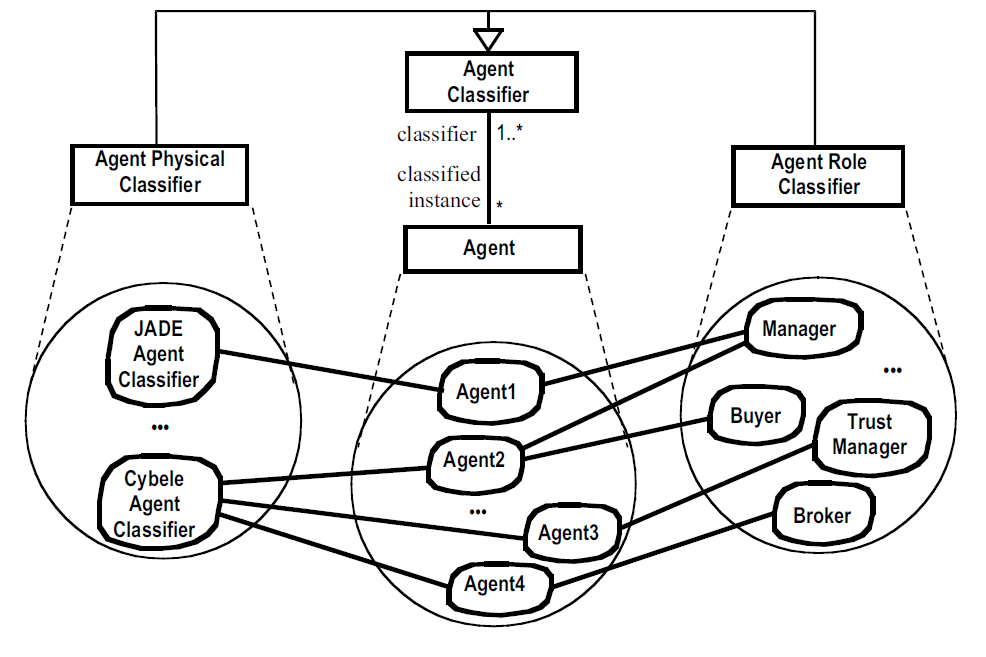
\includegraphics[width=0.75\textwidth]{images/onp/agent-agent-classifier-association.png}
	\caption{The association between \textsc{Agent} and \textsc{Agent Classifiers}}
	\label{figure:onp-agent-agent-classifier-association}
\end{figure}

% Physical vs. role classification
Observe the two main differences between the physical and role classification. First, the role classification is \textit{multiple} whereas the physical classification is \textit{single}.
While an agent can be classified with more than one (or even none) role classifiers at the same time, it must be classified with exactly one physical classifiers.
Second, the role classification is \textit{dynamic} in contrast to physical classification, which is \textit{static}.
Dynamic classification means that an agent can be declassified or reclassified with another role after initial classification. On the contrary, the physical classification is invariable in time
(``Once a JADE agent, always a JADE agent.'').

%%%%%%%%%%%%%%%%%%%%%%%%%%%%%%%%%%%%%%%%%%%%%%%%%%%%%%%%%%%%%%%%%%%%%%%%%%%%%%%%
\subsection{Group, Agentified Group and Non-agentified Group}

% Group - definition
A \textit{group} is a set of agents that are related via their roles, where these links must form
a connected graph within the group \cite{Odell05}.
This is the agent-centric way to look at at a group.
Another way of looking at a group is the role-centric way, which says that a group is a composite structure consisting of interrelated roles, where each of the group's roles has any number of agent instances \cite{Odell05}.

% Group - motivation
A group can be formed to exploit the synergies of its members, resulting in an entity capable of performing processes that none of its constituent agents (ALT: constituents) is capable.

\subsubsection*{Group Metamodel}

Figure~\ref{figure:onp-group} shows the \textsc{Group} class and its associations with \textsc{Agent} and \textsc{Role}.
The abstract \textsc{Group} class extends the UML Structured Classifier, which means that \textsc{Group} is defined as composite structure \footnote{In UML, Structured Classifier can be thought of as a structured set of classifiers. From this perspective, \textsc{Group} is a structured set of \textsc{Agent Role Classifiers}}.

% Figure: Group
\begin{figure}[ht]
	\centering
	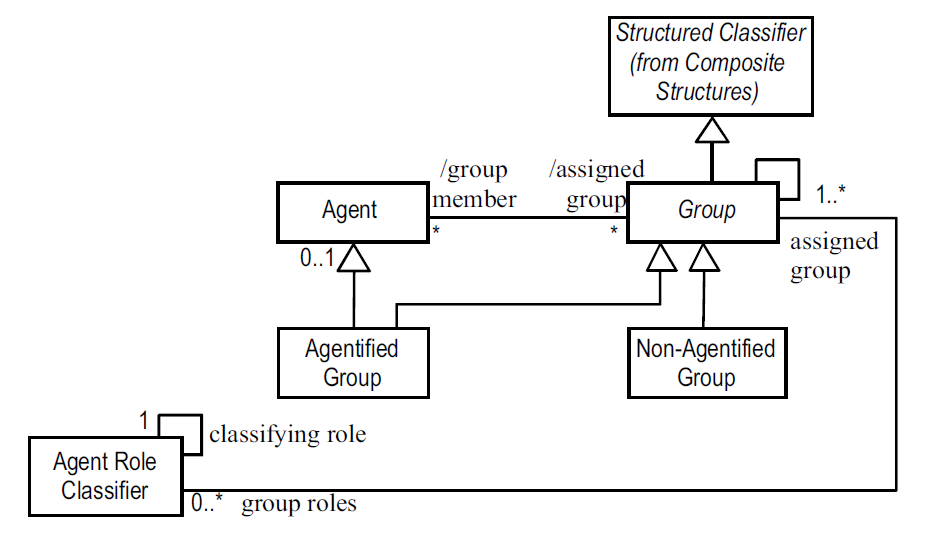
\includegraphics[width=0.75\textwidth]{images/onp/group.png}
	\caption{The \textsc{Group} class and its associations}
	\label{figure:onp-group}
\end{figure}

% Association between Group and Agent
Conceptually, a group consists of a set of agents playing roles within this group.
The roles that the agents can play (within this group) are represented by one or more agent role classifiers associated with this group.
Therefore, the set of agents comprising a group can be derived from the group via the agent role classifiers \cite{Odell05}.

\subsubsection*{Association between Group and Role}

% Association between Group and Agent Role Classifier
Figure~\ref{figure:onp-group-role-association} illustrates the association between groups and roles played in them by agents.
Observe that groups containing no roles is not allowed, each group must contain at least one role.
The opposite direction of the association requires each role to be contained in at least one group, since roles only make sense within context of a group.

% Figure: Group to Role association
\begin{figure}[ht]
	\centering
	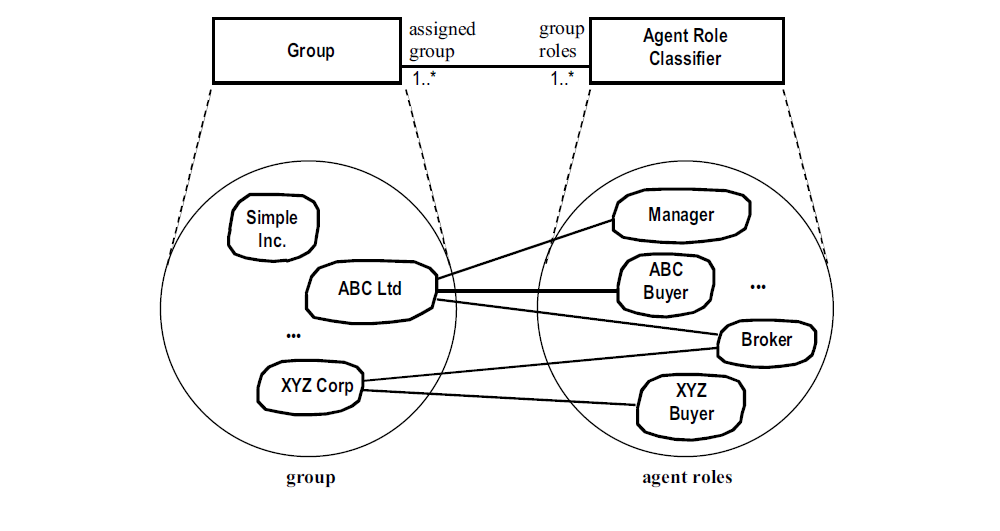
\includegraphics[width=0.75\textwidth]{images/onp/group-role-association.png}
	\caption{The association between \textsc{Group} and \textsc{Role}}
	\label{figure:onp-group-role-association}
\end{figure}

\subsubsection*{Agentified and Non-Agentified Groups}

The O\&P metamodel defines two types of groups: agentified and non-agentified.

% Agentified group
An \textit{agentified group} is a group that is also an agent in its own right, i.e. with its own interactive capability \cite{Odell05}.
This means that an agentified group can communicate with other agents (or agentified groups for that matter) directly, i.e. without a representative agent.
It can also be a member of other groups (agentified or not) and play roles, like any other agent.
To achieve this in the O\&P metamodel, \textsc{Agentified Group} is a subclass of both \textsc{Group} and \textsc{Agent} classes.
Figure~\ref{figure:onp-agentified-group} shows an example of an agentified group.
Notice the <<agent>> stereotype used to mark the group as agentified.

% Figure: agentified group
\begin{figure}[ht]
	\centering
	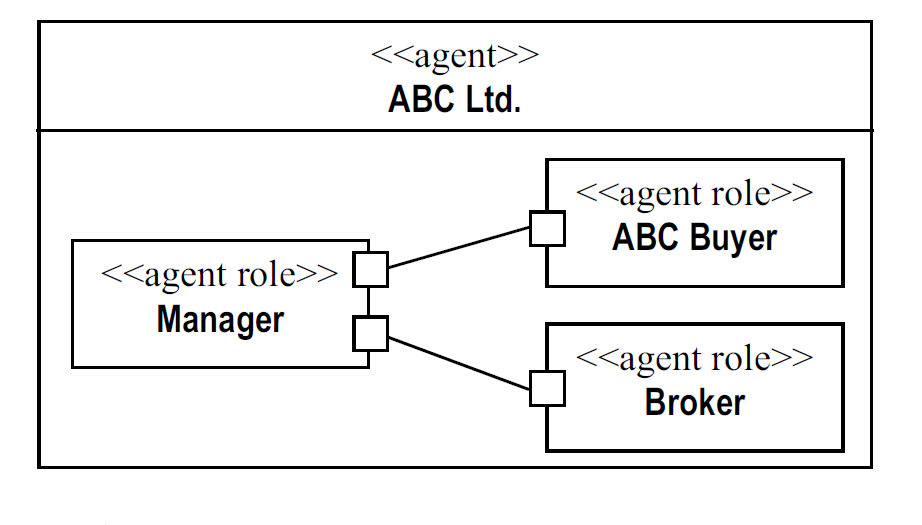
\includegraphics[width=0.5\textwidth]{images/onp/agentified-group.png}
	\caption{An example of an agentified group}
	\label{figure:onp-agentified-group}
\end{figure}

% Non-agentified group
A \textit{non-agentified group}, while still being a first-class citizen, is not an agent by itself, i.e. is it does not posses any capability to interact.
This kind of group always communicates with other agents (including agentified groups) through one of its members acting as an intermediary.
This is achieved in the O\&P metamodel by \textsc{Non-Agentified Group} extending only the \textsc{Group} class and not the \textsc{Agent} class.
An example of a non-agentified group is shown in figure~\ref{figure:onp-non-agentified-group}.
Note that this time there is no <<agent>> stereotype marking the group as agentified.

% Figure: non-agentified group
\begin{figure}[ht]
	\centering
	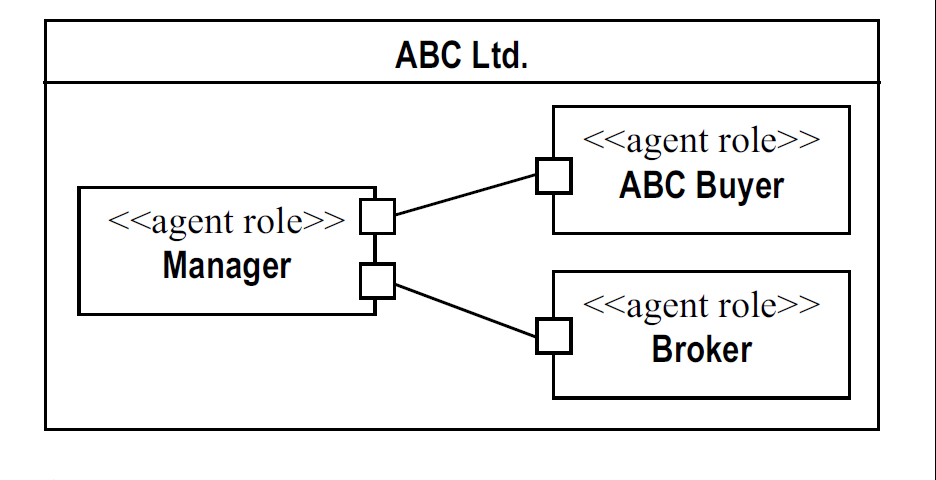
\includegraphics[width=0.5\textwidth]{images/onp/non-agentified-group.png}
	\caption{An example of a non-agentified group}
	\label{figure:onp-non-agentified-group}
\end{figure}

%%%%%%%%%%%%%%%%%%%%%%%%%%%%%%%%%%%%%%%%%%%%%%%%%%%%%%%%%%%%%%%%%%%%%%%%%%%%%%%%
\subsection{Agent Role Assignment}

The assignment of roles to agents is dynamic, i.e. it changes in time, and is modelled by \textit{Agent Role Assignment}.
Figure~\ref{figure:onp-agent-role-assignment} shows Agent Role Assignment and its associations.  

% Figure: Agent Role Assignment class
\begin{figure}[ht]
	\centering
	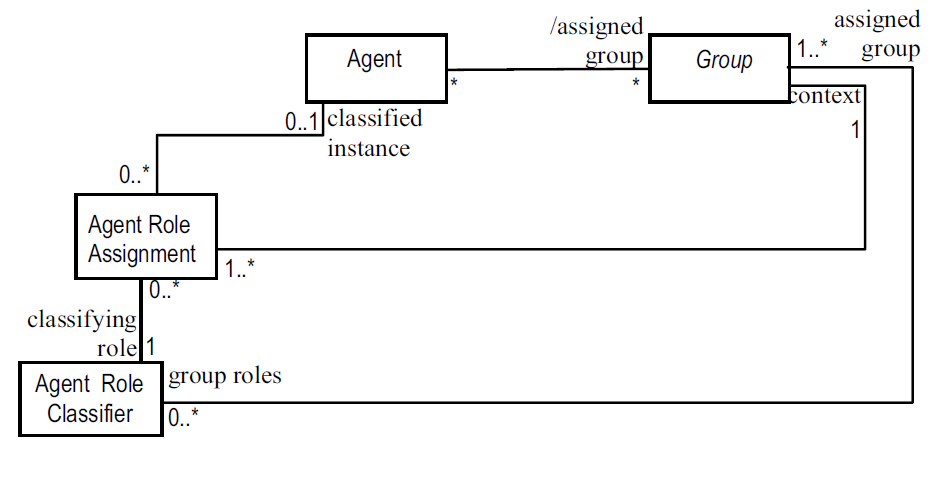
\includegraphics[width=0.75\textwidth]{images/onp/agent-role-assignment.png}
	\caption{The \textsc{Agent Role Assignment} class and its associations}
	\label{figure:onp-agent-role-assignment}
\end{figure}

\subsubsection*{Agent Role Assignment as a Ternary Association}

A direct association between Agent and Agent Role Classifier would represent that agents play roles.
However, such model would not be able to represent a situation where an agent plays a role in one group and does not play it in another.
To model this kind of situations, it is necessary to augment the agent-to-role association with a group context.
This yields a ternary association, promoted to (ALT: reified as) the Agent Role Assignment class.
Each instance of the Agent Role Assignment class associates an agent, role and a group.

\subsubsection*{Position}

It is possible to associate a group with a role leaving out an agent.
Such association is called a \textit{position} and models a situation where a concrete agent playing a role within a particular group is yet to be determined.
This turns out to be an extremely useful modelling concept, since more often than not, the organization modeller does not know (or simply does not care) which agent actually takes up a particular position when the MAS is run.
One more way to look at the \textsc{Agent Role Assignment} class is to view it as a reified association between the (potential) \textsc{Position} and \textsc{Agent} classes.